\chapter{Introduction}\label{ch:introduction}


\instructionsintroduction



\section{High-throughput data and the system biology}

% DNA - DNA structure - automated sequencing - 1st genome - microarray
% - human genome - high-thoughtput era - system biology
% \cite{Westerhoff2004} Figure 1

Molecular biology has dominated the biology research in the past
century with exciting progresses: the discovery of DNA and its
structure, the revelation of the central dogma, the disclosure of
message RNA.
%, has greatly advanced out understanding of living beings.
%
%% Avery started this journey by discovering DNA.  Then the double helix
%% structure of DNA was decoded in 1953 by Watson and Crick.  Next Crisk
%% purposed the central dogma of molecular biology in 1957, which has
%% since been the center of the research.
%
Accompanied by the proliferate developments in biotechnology like the
recombinant DNA technology, the polymerase chain reaction, and the DNA
sequencing, these processes of replication, transcription, and
translation have been extensively studied.
%
Due to the technological limitations, the molecular biologist has
taken a reductionist approach to study a handful of genes or even
single gene in isolation to uncover their connections with the
observable characters of an organism (phenotype).
%
However, ever since the discovery of the complex regulation mechanism
of Lac operon \cite{Jacob1961}, there has been a growing understanding
that an organism is a complex system whose characteristics and behaviors are
often driven by complicated interactions among its components instead
of single gene.  
%
\todo{INTRO [pending]: A better reference for biology as a complex system}
%
Yet, the early efforts were hampered by the lack of experimental
technologies to harvest the data required to study an organism at the
system level.


Heralding the coming high-throughput era, two technological
breakthroughs in 90s dramatically improved our data collection
ability, and revolutionized the molecular biology research.
%
First, automated DNA sequencers emerged and soon reached genome-scale
sequencing \cite{Fleischmann1995}, enabling, for the first time, the
study of the complete genetic material and the discovery of the full
gene universe of a species.
%
%% With the advance of the automated DNA sequencing technology, the first
%% complete genome of an organism was sequenced in 1995, and in 2001, the
%% draft genome of human was released.
%% %
%% The avaiability of the complete genetic material of a species coupled
%% with the developments in functional genomics generated, for the first
%% time, the total universe of genes for one organism.  This reveals what
%% a small part of this world is known, and how much still remains to be
%% explored.
%
This is followed by the development of the microarray technologies
\cite{Pease1994, Schena1995} that was utilized first to study the gene
expression at genome-scale \cite{Davis1997}, and later to generate
additional `omics' data types \cite{Blat1999, Uetz2000}.
% \cite{Brown1999} for more references if needed
%
Due to their unprecedented ability, accompanied by the swift
developments of required computational tools, these technologies were
broadly adopted in biology researches, and shortly in a scaled-up
settings \cite{Su2002,Su2004}.
%
The availability of various types of data for an organism at genome-scale
finally expedited the emergence of system biology as an approach to biological
research.  System level models of interacting components are constructed in
order to provide insights into the function and control of biological systems
that are not apparent from studying the individual component, and in turn, to
generate experimentally verifiable hypotheses that deepen our understanding of
those systems \cite{Ideker2001, Palsson2002}.
%
The advance in system biology commands ever more comprehensive data set.
However the amount of data generated by individual experiment is physically
constrained by the number of biological samples tested, whereas a colossal
volume of gene expression experiments are publicly available but largely remain
underutilized.
%
The research presented in this dissertation aims on bridging this gap
by developing a methodology to construct comprehensive
organism-specific expression compendia through a direct integration of
publicly available experiment data.
%
%\todo{Carolina: you think it is better to remove this part from here?}

%% \textbf{Systems Biology} as an approach to biological research that
%% studies biological systems and processes as dynamic, integrated
%% networks of interacting molecules 
%% %
%% The underlying vision is that the structure and dynamics of such
%% networks will provide insights into the function and control of
%% biological systems that are not apparent from studying the systems'
%% components.


%% [HUI Thesis p1]
%
%% A biological system is not just an assembly of genes or proteins and
%% their interconnections. It can be understood at different levels such
%% as cells, tissues, organs and organisms. These are all systems of
%% components whose specific interactions have been defined by evolution.
%% %
%% Therefore, while the understanding of individual genes and proteins
%% continues to be important, the system-level understanding will help us
%% gain more insight in the complexity of a biological system.
%% %
%% Systems biology emerged in this respect. Systems biology does not
%% investigate individual genes or proteins one at a time. It
%% investigates the behaviour and interactions of all the components in a
%% particular biological system while it is functioning [1].
%% %
%% The development of systems biology has been driven by obtaining,
%% integrating and analyzing high-throughput data from various
%% experimental sources. These high-throughput biological experiments
%% supply thousands of measurements per sample and generate
%% high-throughput data to be used to enhance inference at a system
%% level.


%% [RIET Thesis p2]
%
%% The emergence of high-throughput technologies, such as genome
%% sequencing technologies and microarrays, has lead to an explosion of
%% complex and noisy data.
%% %
%% To understand the underlying biology of these data, systems biology is
%% relying on an intimate integration of both mathematical and biological
%% methods.
%% %
%% The novel field of bioinformatics or computational biology is
%% concerned with the development of data mining tools that are
%% specifically designed to translate complex biological data into novel
%% biological insights and that can be used interchangeably with
%% experimental procedures to validate the predictions.
%% %
%% This field covers a broad range of biological topics, such as gene
%% function prediction, cis-regulatory motif detection, network
%% prediction, gene evolution etc.










\section{Microarrays and data preprocessing}

%% \textbf{The emerge of microarray}
Fundamentally hybridization based, the microarray technology has its root in
Southern blotting, where fragmented DNA attached to a substrate are probed with
a known DNA sequence.
%
Although the earliest approach that resembles microarray appeared in
80s \cite{Augenlicht1982}, it is not until large amount of sequences
became available following the advances in the automated sequencing
technology that a microarray capable of probing thousands of genes'
expression simultaneously has become possible.
%
And the first genome-scale microarray for \textit{Saccharomyces
  cerevisiae} \cite{Davis1997} appeared shortly after its complete
genome sequence was released \cite{Goffeau1996}.
%
With its unprecedented ability, microarray has quickly become an
indispensable technology to quantify global gene expressions.


%% \textbf{Microarray technologies}
There are different microarray platforms for measuring gene expression, such as
Affymetrix, Agilent, Nimblegen, or in-house microarrays \cite{Sasik2004}.
%% %
%% They can be classified in two categories by the manufacturing
%% technologies, namely, spotted array and \textit{in situ} synthesized
%% array.
%% %
%% The spotted array is produced by spotting pre-synthesized DNA probes
%% corresponding to specific genes on a solid surface.  Typically, the
%% probes can be oligonucleotides (usually 50-80 bases), long
%% complementary DNA strains (100-1000 bases), or small fragments of PCR
%% products.
%% %
%% For \textit{in situ} synthesized array, the probes, each of which is a
%% short sequence designed to target a specific gene or family of gene
%% splice-variants, are syntehsized directly on the chip surface.
%% %
%% Alternatively, the microarray 
They can be categorized according to the number of samples that can be
hybridized simultaneous on a chip.
%
\textit{Two-channel microarrays} or \textit{dual-channel microarrays}
are typically hybridized with cDNA prepared from two samples and
labeled with two different fluorophores (commonly Cy3 with green
color and Cy5 with red color).
%
Relative intensities of each fluorophore (color channel) are used to calculate
ratios representing gene expression changes to identify up-regulated and
down-regulated genes between samples.
%
Typical example of dual-channel microarrays are cDNA arrays whose
probes are cDNAs synthesized from mRNAs.
%
In \textit{one-channel microarrays} or \textit{single-channel
  microarrays}, only one sample is hybridized to a chip generating
intensity data for each probe or probeset.
%
However these intensities do not reflect the absolute abundance levels of a
gene but rather the relative ones when compared to other samples or conditions
processed in the same experiment, as the experimental protocol and
batch-specific biases render a direct comparison of gene's intensities of same
platform origin across experiments uninformative.
%
Affymetrix ``Gene Chip'', the most popular one of such platforms due to its
high accuracy and precision \cite{Irizarry2005}, is used as an example to
discuss the issues related to this type of arrays.


%% \textbf{Microarray data processing}
Microarray data are very noisy.  There are many sources of systematic variation
in microarray experiments that affect the measured gene expression levels, such
as, heat and light sensitivity, dye labeling and detection efficiency, and
unequal quantities of starting RNA, etc \cite{Kerr2001,Zakharkin2005}.
%
It is crucial to apply normalization procedures on raw expression intensities
to remove systematic bias arising from the variations in the microarray
technology rather than from biological differences between samples 
\cite{Quackenbush2002}.
%
Various methods have been developed for this purpose, and most are platform
dependent.

For cDNA microarray, the log-ratios calculated from the per-channel intensities
from the same spot (probe) theoretically negate most of the systematic noises
related to manufacture variations, such as, spot effect, print-tip effect, etc.
%
However, often there exists intensity dependent artifacts in the obtained
log-ratios which can be visualized in a MA plot \cite{Yang2002}.
%
Locally weighted linear regression (LOWESS) analysis \cite{Cleveland1979} first
proposed by Yang \textit{et al.} \cite{Yang2002} has been shown to successfully
remove such artifacts, and became the most widely used normalization method for
cDNA microarray.
%
This method was later replaced by LOESS (LOcal regrESSion) which is more
flexible albeit computationally more intensive.
% We refer the reader to \cite{Quackenbush2002} for a through review of cDNA
% microarray preprocessing.
%
%%  Check Quackenbush2002 for more details !!!

For single-channel microarray, such as, Affymetrix platform, a desirable
normalization method needs to remove all variations of non-biological origin
across arrays, as each array generates relative gene expression intensities for
one sample only, whereas gene expressions of different samples (produced on
different arrays) must be made comparable to observe true variations originated
from biological differences between samples.
\todo{INTRO [pending]: explain the probe probeset...}
%
Among the large number of methods developed for the popular Affymetrix
platform, a global quantile normalization \cite{Bolstad2003,Irizarry2003a}
coupled with medial polish summarization \cite{Irizarry2003}, combinedly known
as robust multi-array average (RMA) method, has been shown to outperform other
methods \cite{Irizarry2006} providing better precision even with few biological
replicates.  It soon became the \textit{de facto} standard normalization
method for this platform.
%
% \cite{Do2006} minireview of normalization








\section{Gene expression compendium}
%
\todo{INTRO [pending]: historical perspective for compendium}


%% from Hui thesis 2.3 introduction
%
%% Microarray technology has become an indispensable technology for studying large
%% scale transcriptional gene expression in genomics research.
%% %
%% Increased accessibility, lowered cost and improved technology result in more
%% comprehensive studies, under more diverse and larger sets of conditions and a
%% rapid expansion of available gene expression data. 
%% %
%% Mining from the integrated large scale microarray data offers the molecular
%% biologists the possibility to view their own small scale analysis in the light
%% of what is already available and also the opportunities towards studying in
%% network and pathway perspective.
%% %
%% A first step towards integration the large scale microarray data from different
%% laboratories in different conditions is to generate microarray compendia.


%% (Hui thesis 2.3.1) SKIPPED
%
%% historical perspective, from small-scale to compendium scale microarray
%% experiments
%% ----------------------------------------------------------------------------


%% Microarray (small scale) => Large complex microarray experiment (large
%% scale) => Microarray compendium (global scale) => system biology =>
%% comprehensive dataset - - - > (online repository, next paragraph)

%% Early microarray experiments were usually in small-scale involving a limited
%% number of samples,
%% %%  utilized its potential to probe large number of genes to identify
%% %%  differentially expression ones when comparing two distinct samples
%% %%  \cite{Schena1995, DeRisi1996, DeRisi1997}.
%% %
%% and each microarray was studied in isolation providing only a snapshot of the
%% gene expression changes under specific conditions.
%% %
%% As the scale of the experiment increases, the gene expression patterns and
%% systematic features emerged to become the focus of study \cite{Cho1998,
%%   Marton1998, Spellman1998, Brown1999}.
%% % utilizing existing computational methods \cite{Eisen1998, Tamayo1999}.
%% %
%% Soon large-scale gene expression data set called compendia are generated and
%% utilized to study various biological phenomena at a global scale
%% \cite{Hughes2000, Su2002, Su2004}.
%% %
%% These studies demonstrate that a compendium, which incorporates large number of
%% samples with various properties, complements and extends the data
%% comprehensiveness at gene level provided by microarray technology, enables


%% A new type of biogolical research approach, system biology, 


%% Soon large-scale data set called compendium were systematically generated to
%% augment functional annotation of gene, to study transcriptional regulation, to
%% identify disease marker genes, to analyze parental imprinting, and to study gene
%% conservation by comparing transcription profiles across species
%% \cite{Hughes2000, Su2002, Su2004}.
%% %
%% Alternatively, in Pilpel \textit{et al}. 2001 \cite{Pilpel2001}, expression
%% data originated from different studies are combined to form a comprehensive
%% data set in order to study the combinatory transcriptional regulation and the
%% underlying regulatory network.
%% % \cite{Ren2000} ChIP-on-chip, expression data, combinatory regulation
%% % \cite{Pilpel2001} combined with motif information to study regulatory network (1st)
%% %
%% One common feature of those studies is that harboring large-scale gene
%% expression data set with extensive coverage across variant samples to make new
%% discovery, extending the data comprehensiveness at gene level provided by
%% microarray technology with that at sample level.
%% %
%% Clearly, although one study can amass a great deal of information to analyze a
%% certain aspect of an organism, none can be so comprehensive to cover the
%% organism's full scale of complexity.
%% % \cite{Ideker2001}


%% %% \cite{Hughes2000} 
%% %% - functioanl characterization of unknown genes through profile matching
%% %% - characterize pharmacological perturbation by identifying novel drug target 
%% %% * stressed the issue of a extended compendium (more mutants, various grownth
%% %%   conditions)
%% %
%% %% \cite{Su2002}
%% %% - Affymetrix single-channel intensity based compendium
%% %% - extended scope of the compendium: transcriptional regulation, biomarker
%% %%   identification, cross-species comparison.
%% %
%% %% \cite{Su2004}
%% %% - customized Affymetrix microarray containing uncharacterized genes
%% %% - novel gene imprint




%% %% Check Hui thesis 2.3

%% 1. benefit of data integration, literature studies 

%% 2.1. online repository, data available

%% 2.2. data integration method: Meta-analysis vs compendium

%% 3. Issues with current direct data integration => cross-platform approach
%%    (issues with cross-platform approach are detailed in Chapter 2)




%% Online repository
%% --------------------------------

% Data storage and reuse issue \cite{Baxevanis2001}, early Databases to manage
% yeast expression data \cite{Aach2000, Marc2001}

As microarray become an indispensable technology for studying gene expression,
large amount of data has been generated.
%
To promote data sharing, scientific journals generally require the deposit of
these high-throughput experiments in public databases, such as Gene Expression
Omnibus (GEO) \cite{Barrett2011} or ArrayExpress \cite{Parkinson2009}, upon
publication.
% \cite{Edgar2002} GEO \cite{Brazma2003} ArrayExpress
These databases are an extremely rich source of information, containing freely
accessible data for thousands of experiments and a multitude of different
organisms, and in theory provide an opportunity to analyze gene expression of a
particular species at a global level \cite{Ideker2001}.
%
Additionally, they hold the potential to expand the scope of any smaller scale
study: mining the existing information offers molecular biologists the
possibility to view their own dedicated experiments and analysis in light of
what is already available.



%% \subsection{Benefit of compendium and its applications}
%% The benefit of a comprehenisve data set has long been appreciated since the
%% invention of microarray technology.
%% %% %
%% %% Large-scale gene expression data set called compendia are generated and utilized
%% %% to study various biological phenomena at a global scale \cite{Hughes2000,
%% %%   Su2002, Su2004}.




\subsection{Data integration issues}
%% data integration issues
%% ---------------------------------------------------------------------

\todo{INTRO [pending] Carolina: 
Just a suggestion, it depends how much you talk about probe-gene
mapping...  if you do not mention it, then just ignore the comment.
but another issue is the constant updating of genome annotations. Some
platforms are very old, like the custom cDNAs while commercial
platforms stick to up-to-date genome annotation. the gene annotations
evolve and old probes could be re-annotated and point to other genes
as originally designed.}
%
%% * online repository (thesis Hui 1.2, 2.3 and Riet 1.1.3, 1.1.4 )
%%   (data issue prevents its utility)
%%   - representation issues
%%   - platform differences
%%   - normalization issues
%
However, the opportunity of combining all public experiments for a single
organism has not been explored due to two practical issues, data heterogeneity
and data representation heterogeneity.
%
First, microarray data are inherently highly heterogeneous.
%% However, the opportunity of combining all public experiments for a single
%% organism has not been explored due to practical issues that can ultimately be
%% attributed to the large heterogeneity inherent to microarray data.
%
Data sets originate from different experimenters or labs and microarrays do not
constitute a uniform technology.
%
Even for data generated on one platform, protocols for sample preparation,
labeling, hybridization, and scanning can vary greatly across labs and even
studies, deteriorating the data compatibility \cite{Bammler2005, Irizarry2005}.
%
The consistency among data generated on different platforms is even worse due to
the probe design and manufacture variations \cite{Sasik2004, Draghici2006}.
% probe mapping methods \cite{Mecham2004, Carter2005}
%
%% %% Multiple microarray platforms do exist and are manufactured in different ways
%% %% \cite{Sasik2004}.  This worsened the consistency among data generated across
%% %% different platforms.
%% %
%% %% Various technologies exists to manufacture different types of microarraies, such
%% %% as, cDNA spotted array, Affymetrix, Agilent, Nimblgen, etc
%% %% (\cite{Sasik2004}). [\cite{Fierro2008}]
%
Moreover, the aforementioned platform-dependency of pre-processing methods
% the applicability of data pre-processing methods is platform dependent
further lowers the data coherence, as often, different studies
employ different methods \cite{Irizarry2005, Shi2006, Stafford2007}.
%
%% The platform-dependency of data pre-processing methods coupled with the lack
%% of a golden-standard normalization procedure for each platform further
%% lowered the data coherence, as different studies, unrelated to the platform
%% employed, often employ different ones \cite{Irizarry2005, Shi2006,
%% Stafford2007}.
%
%% Utilizing variant pre-processing methods in different studies further worsened
%% the situation \cite{Irizarry2005, Shi2006, Stafford2007}.
%% %
%% Each different platform requires its own optimized sample preparation,
%% labeling, hybridization and scanning protocol, and concomitantly also a
%% specific normalization procedure. [\cite{Fierro2008}]
%
Second, although community standards specifying the mandatory minimal
experimental information accompanying each dataset (e.g., MIAME
\cite{Brazma2001}) have been long established, the lack of the requirements
\cite{Brazma2009} imposed regarding the format of the platform descriptions and
the expression measurements, as well as the degree of preprocessing done on
these values further complicates the matter of experiment integration from a
practical point of view.
%
%% Consequently, data are segregated per experiment due to the lack of uniformity
%% in reporting expression data, the heterogeneity of the microarray platforms, and
%% the incomplete and inconsistent meta information specifying experimental
%% conditions.




\subsection{Existing compendium construction efforts}

%% existing efforts: meta-analysis .vs. single platform direct integration
%% --------------------------------------------------------
Despite such difficulties, several initiatives exist to actively build
expression compendia from public resources.
%
%% Most existing compendia can roughly be divided in two groups \cite{Fierro2008}:
%% those that directly integrate single-platform experiments, and those that
%% indirectly integrate cross-platform experiments.
Reviewed in Fierro \textit{et al.} \cite{Fierro2008}, the existing compendia
took two different approaches to alleviate the aforementioned data integration
issues: directly integrating data across experiments albeit limited by only
those generated on a single-platform \cite{Faith2008, Hruz2008}, or combining
results of individual experiment through meta-analysis to avoid direct data
integration across experiments \cite{Rhodes2007, Pan2007, Elfilali2006,
  Kapushesky2010, Culhane2012}.



%% \textbf{meta-analysis}
%% ------------------------------------------------------------
Meta-analysis is capable of combining data from different experiments across
variant platforms, albeit in an indirect manner.
%
%% Combining data from different platforms, even to the extent of combining data
%% from single- and dual-channel microarrays, is generally done by indirect
%% meta-analysis as opposed to directly integrating the actual expression values:
It is generally a two step analysis: one first applies the desired analysis
procedure (e.g., identifying differentially expressed genes, clustering gene
expression profiles, etc.) on each single data set within the compendium
separately, and subsequently combines the derived results.
%
These compendia are often topic-specific, collecting all publicly available
experimental information related to a subject matter of interest.  ITTACA
\cite{Elfilali2006} and ONCOMINE \cite{Rhodes2007}, for instance, focus on
cancer in human; Gene Aging Nexus \cite{Pan2007} on aging in several species;
GeneSigDB for gene signatures of cancer and related diseases \cite{Culhane2012}.
%
Exceptionally, the ATLAS \cite{Kapushesky2010} initiative from ArrayExpress
provides gene expression meta-analysis data sets for several species.  However,
containing only 400 experiments over all species in total and biased towards
several eukaryotic model organisms, it is still far from comprehensive.
%% There are exceptions though, such as the large ATLAS \cite{Kapushesky2010}
%% initiative from ArrayExpress. 

%% INMEX \cite{Xia2013} webservice to perform meta-analysis, not compendium



%% \textbf{direct integration}
%% ------------------------------------------------------------
Alternatively, the direct integration approach removes data heterogeneity by
applying normalization method across studies, then merges the results together
to form one expression data set.
%
Ideally, all data publicly available for a species could be integrated into
one comprehensive compendium.
%
Due to the aforementioned issues, the existing ones, however, focus on gathering
only the data generated by single platform, for instance, M$^{\textrm{3D}}$
\cite{Faith2008} or the commercial Genevestigator \cite{Hruz2008}.
%
The Affymetrix platforms is often chosen as the target platform, as they are the
most widely used ones due to their robustness and high reproducibility
\cite{Bammler2005, Irizarry2005}.
%
The single-channel nature of the Affymetrix platform and the use of proprietary
file formats to report platform information and expression measurements avoid
the data representation heterogeneity that plagues the data generated by many
other platforms, and make the data collection task straightforward.
%
Combining data from a single platform makes the in-between experiment
normalization and probe mapping relatively straightforward, so that the
quantitative measures of gene expression can be analyzed directly across
experiments.
%
%% Most single-platform compendia databases, such as for instance M$^{\textrm{3D}}$
%% \cite{Faith2008}, or the commercial Genevestigator \cite{Hruz2008}, focus on
%% Affymetrix, one of the more robust and reproducible platforms \cite{Bammler2005,
%%   Irizarry2005}.  
%
%% Why cross-platform
For eukaryotic model organisms, such a single-platform approach works well as
the compendium based on Affymetrix chips can achieve a broad scope on
experimental condition due to the platforms popularity.
%
For instance, Lukk \textit{et al.} \cite{Lukk2010} created a comprehensive data
set for human containing 5372 microarrays representing 369 different cell and
tissue types, disease states and cell lines.
%
For prokaryote, however, the single-platform constraint severely circumscribes
the scope of the compendium created due to the lack of such a dominate platform.
%
Even for a widely studied model organism, such as {\it E. coli}, the most 
popular platform `Affymetrix GeneChip E. coli Genome 2.0 Array' is used in less 
then one thirds of all publicly available experiments.
%
When considering only one platform, a significant portion of data is missed out 
on.  A novel approach that can integrate data of different platform origin is 
highly desirable.



%% \textbf{Comparison meta-analysis and direct integration}
%
When combining data from multiple experiments that address a set of related
research questions, both meta-analysis and direct data integration approaches
enjoy the benefit of higher statistical power and more robust inference due to
the increased number of samples in the combined data set and the reduced effect
of study-specific biases \cite{Sutton2001, Xu2005, Warnat2005}.
%
%% From a statistical point of view, such meta-analysis is interesting as for
%% single experiments the number of replicated conditions is usually small. By
%% combining results from different studies that address \textbf{a set of
%% related research hypotheses}, the number of replicates and the power of the
%% statistical tests will increase \cite{Sutton2001}.  [carolina]
%
%% It is of great interest to integrate inter-study microarray data to increase
%% sample size, which could lead to the discovery of more reliable or novel
%% markers \cite{Xu2005}.
However, when compared to direct data integration, meta-analysis approach has
several disadvantages.
%
First, the meta-analysis approach can only generalize those biological
findings which are statistically significant in a high enough number
of individual studies.  This results a great lose of information, and
consequently leads to high false-negative rates \cite{Lazar2012, Xu2008}.
%
It has been observed that when compare meta-analysis and direct analysis of
integrated data for differential expressed gene retrieval, taking the results
obtained by the analysis of a single experiments as a reference, direct analysis
of multiple experiments detects more differentially expressed genes while
indirect analysis tend to result in a more restricted gene list which
corresponds \textit{grosso modo} to the intersection of the sets of
differentially expressed genes obtained by each of the single experiments
\cite{Fierro2008}.
%
On the contrary, all the data are retained in the direct integration approach.
New discovery can be generated when the combined data are analyzed together.
%
Indeed, Warnat \textit{et al.} \cite{Warnat2005} shows that direct integration
reveals novel genes that is otherwise missed in single-set analysis, and the
classifier incorporating those genes shows high predictive power and improved
generalization performance.
%
Second, the compendium based on meta-analysis are limited by the predefined
functionalities provided by the system, hence lack of flexibility to incorporate
new analysis.  
%
The ones created by direct integration, however, retain actual expression
values, hence the compendia can be readily analyzed by the existing and
potential methods.  This greatly broadens the scope of the utility of the
compendium.
%
For example, the \textit{E. coli} compendium of M$^{\textrm{3D}}$
\cite{Faith2008}, which is originally created to study transcriptional
regulation in this species, has been applied to benchmark network inference
algorithm \cite{Marbach2012}, to discover conserved biclusters across multiple
species \cite{Kacmarczyk2011}, and to study chromosome conformation alternations
under different physiological conditions \cite{Ma2013}, etc.
%
%\todo{INTRODUCTION: check Taminau2014}


%% %% Advantages of data integration
%
%% From a statistical point of view, such meta-analysis is interesting as for
%% single experiments the number of replicated conditions is usually small. By
%% combining results from different studies that address \textbf{a set of
%% related research hypotheses}, the number of replicates and the power of the
%% statistical tests will increase \cite{Sutton2001}.  [carolina]
%
%% It is of great interest to integrate inter-study microarray data to increase
%% sample size, which could lead to the discovery of more reliable or novel
%% markers \cite{Xu2005}.

%% %% --------- meta analysis limitations 1
%% meta-analysis (differential expressed gene only, not the full gene)

%% When compare meta-analysis and direct analysis of integrated data for
%% differential expressed gene retrieval, taking the results obtained by the
%% analysis of a single experiments as a reference, direct analysis of multiple
%% experiments detects more differentially expressed genes while indirect analysis
%% tend to result in a more restricted gene list which corresponds grosso modo to
%% the intersection of the sets of differentially expressed genes obtained by each
%% of the single experiments \cite{Fierro2008}

%% \cite{Lazar2012} 
%% %
%% Only biological findings that are found as being statistical significant in a
%% high enough number of individual studies can be used for generalization.
%% %
%% the overall statistical analysis will suffer from the insufficient number of
%% samples (due to different practical limitations in the design of the
%% experiments) processed in each individual experiment, which leads to high
%% false-negative rates.
%% %
%% the analysis of datasets containing few samples is the fact that the statistical
%% hypothesis tests used to make decisions ware prone to high false-negative rates.

%% The major limitation of meta-analyses is that the sample sizes
%% typical of individual studies, coupled with variation due to
%% differences in study protocols, inevitably degrades the results.
%% %
%% Also, deriving separate statistics and then averaging is often less
%% powerful than directly computing statistics from aggregated data
%% \cite{Xu2008}.


%% %% --------- meta-analysis limitations 2
%% Last, compendia created in this manner are limited by the predefined
%% functionalities provided by the system, hence lack of flexibility to incorporate
%% new analysis.



%% %% --------- direct integration: advantages
%% The compendia created by direct integration, however, retain actual expression
%% values, hence the compendia can be readily analyzed by the existing and
%% potential methods.
%% %
%% The compendia created by directly integrating data across experiments have
%% the advantage of retaining actual expression values, which broadens the scope
%% of potential analysis procedures compared to indirect meta-analysis.

%% Direct integration reveals novel genes that is otherwise missed in single-set
%% analysis, showing high predictive power and improved generalization performance
%% \cite{Warnat2005}.

%% An obvious advantage of an integrated classification analysis is the improved
%% generalization performance and reliability of the resulting predictive models
%% (classifiers) since they are found and validated on a larger number of samples,
%% thus the effect of study-specific biases can be reduced \cite{Warnat2005}.

%% It is of great interest to integrate inter-study microarray data to increase
%% sample size, which could lead to the discovery of more reliable or novel markers
%% \cite{Xu2005}.

%% \cite{Pilpel2001}









%% \textbf{COLOMBOS}
%% Existing compendia alleviate the aforementioned data integration issues by 
%% either directly integrating data across experiments albeit limited by only 
%% those generated on a single-platform \cite{Faith2008, Hruz2008} 
%% or combining results of individual experiment through meta-analysis to avoid 
%% direct data integration across experiments 
%% \cite{Rhodes2007, Pan2007, Elfilali2006, Kapushesky2010}.
%% Compendia created by meta-analysis are limited by the predefined  
%% functionalities provided by the system, hence lack of flexibility to 
%% incorporate new analysis.
%% The compendia created by direct integration, however, retain actual expression 
%% values, hence the compendia can be readily analyzed by the existing and 
%% potential methods.
%% For eukaryotic model organisms, such a single-platform approach works well 
%% as the compendium based on Affymetrix chips can achieve a broad scope on 
%% experimental condition due to the platforms popularity.
%% For prokryote, however, the single-platform constraint severely 
%%circumscribes 
%% the scope of the compendium created due to the lack of such a dominate platform.
%% For example, for model organisms such as {\it E. coli}, even the most popular 
%% platform `Affymetrix GeneChip E. coli Genome 2.0 Array' is used by less then 
%% one thirds of experiments. A significant portion of data is missed out on 
%% when considering only one platform.







%% % integrated into the discussion of direct integration approach
%% % (above)
%
%% \subsection{Cross-platform expression compendium}

%% The single-platform approach works well for eukaryotic model organisms as
%% %% Why cross-platform
%% %% For eukaryotic model organisms, such a single-platform approach works well as
%% the compendium based on Affymetrix chips can achieve a broad scope on
%% experimental condition due to the platforms popularity.
%% %
%% For instance, Lukk \textit{et al.} \cite{Lukk2010} created a comprehensive data
%% set for human containing 5372 microarrays representing 369 different cell and
%% tissue types, disease states and cell lines.
%% %
%% For prokaryote, however, the single-platform constraint severely 
%%circumscribes
%% the scope of the compendium created due to the lack of such a dominate platform.
%% %
%% Even for a widely studies model organism such as {\it E. coli}, the most popular
%% platform `Affymetrix GeneChip E. coli Genome 2.0 Array' is used by less then one
%% thirds of experiments.  A significant portion of data is missed out on when
%% considering only one platform.
%% %
%% A novel approach that can integrate data of different platform origin is highly
%% desirable.

%% \paragraph{feasibility}
%
%% \cite{Fierro2008}
%% %
%% All these differences complicate the meta-analysis of arrays performed in
%% different research groups. Several studies have evaluated the feasibility of
%% cross-platform and cross-laboratory integration of array experiments.  While
%% some studies show low reproducibility of expression ratios between different
%% studies \cite{Bammler2005, Tan2003}, others present more promising results
%% \cite{Kuo2006, Sasik2004} .  Irrespective of their final conclusion, these
%% comparative studies revealed the most important \textbf{factors to be addressed
%%   when aiming at integrating data from different studies}.





\todo{INTRO [pending]: Applications of large-scale heterogeneous compendium}
%% \subsection{Applications for large-scale heterogeneous compendium}

%% aka Benefit of data integration


%% \cite{Lazar2012}
%% %
%% The higher statistical relevance of the results obtained by analysing datasets
%% of hundreds or thousands of samples which naturally leads to more robust
%% inference.
%% %
%% % NOTE: for gathering similar data sets only, might not applicable to large
%% %       hetergeneous compendium as a whole !!!
%% %
%% Robust statistical parameters that could lead to robust inference can only be
%% estimated from a large population of samples.  Combining datasets from different
%% sources will result in larger datasets which will provide more statistical power
%% for the subsequent analysis by a more robust estimation of the different
%% statistical parameters required.

%% From a statistical point of view, such meta-analysis is interesting as for
%% single experiments the number of replicated conditions is usually small. By
%% combining results from different studies that address \textbf{a set of related
%%   research hypotheses}, the number of replicates and the power of the
%% statistical tests will increase \cite{Sutton2001}.  [carolina]




%% \cite{Parkinson2009} ATLAS1 p3
%% The meta-analyses indicate that despite these data originating from multiple 
%% laboratories, the biological signal in these data is significantly stronger 
%% than the laboratory effects and new biological insights can be obtained from 
%% this approach.

%% \cite{Zimmermann2004} GENEVESTIGATOR1 p5
%% The general hypothesis in our approach is that as the number of experiments 
%% per category (e.g. growth stage 5.10) increases, individual effects are 
%% averaged out and global trends become visible.


%% 1. compendium to benefit both system biology research and the molecular biology
%% research (\cite{Ideker2001} see section 1.1)


%% 2. \paragraph{why data integration for data exploration ?}\cite{Fierro2008}

%% Many independently performed experiments exist in which a similar process is
%% studied in comparable conditions, for example for the profiling of gene
%% expression in a specific cancer type. Such datasets are ideally suited for the
%% indirect meta-analysis of genes that are differentially expressed between two
%% biological conditions. Rhodes et al. \cite{Rhodes2002} combined four
%% independent datasets to identify genes dysregulated in prostate
%% cancer. However, it is still limited in its use as it requires that the
%% different datasets which are combined test the exact same conditions.

%% To extend this approach to a compendium of more heterogeneous conditions,
%% Rhodes et al. \cite{Rhodes2004} first subdivided the compendium in subsets
%% according to predefined comparisons of interest (e.g., cancer versus normal,
%% undifferentiated versus well differentiated cancer). By searching for subsets
%% of genes that are frequently differentially expressed in a subset, but not
%% necessarily in all the conditions within the subset they introduced more
%% flexibility towards the heterogeneity of the data.


%% 3. \cite{Shi2008, Shi2006}

%% hypothesis-driven biological research \cite{Ideker2001, Kitano2002}


%% 4. \paragraph{the advantage of systemmetical analysis at large scale}

%% Given the complexity of a living cell and its interaction with the environment,
%% it has been shown that computational analysis of \textit{large-scale} dataset
%% across diverse experimental conditions and cell types is a powerful tool to
%% reverse engineer regulatory networks \cite{Faith2007, Basso2005, Ernst2008}, to
%% study its condition dependent behavior \cite{Lemmens2009, Fadda2009}, and to
%% identify compound mode of action \cite{Gardner2003, Basso2005, DiBernardo2005}.
%% % from Faith paper
%% Compendium to study compound mode of action \cite{Gardner2003, Basso2005,
%%   DiBernardo2005} for drug compounds screening to distinguish the molecular
%% targets of bioactive compound from genes indirectly influenced.

%% % \cite{Ideker2001} System Biology
%% Although individual researchers may amass a great deal of knowledge about the
%% genes, molecular interactions, and other biological information underlying one
%% particular pathway, no single biologist can be familiar with the extremely large
%% and complex number of interactions in an entire cell. (p350)
%% %
%% It would be highly desirable to analyze expression levels and other global
%% measurements in a way that validates our current knowledge of a cellular process
%% and isolates discrepancies between expected and observed levels (p351)

%% Several studies showed that classifiers trained with a compendium outperform
%% classifiers based on a single dataset \cite{Warnat2005, Xu2005}.

%% Reconstruction of co-expression network and TRN (co-expression co-regulation)
%% \cite{Choi2005,Yan2007,Huang2007,Faith2007,Ucar2007}

%% Biclustering and module inference (Hui en Riet thesis)

%% Another application is the clustering of genes that share a similar gene
%% expression pattern across the tested conditions.  Hetergeneous compendium,
%% overlap condition dependent co-expression bicluster of global analysis
%% \cite{DenBulcke2006, Lemmens2006, Lemmens2009, Zhao2011}, or through query
%% driven approaches \cite{Dhollander2007,Hibbs2007}.


%% Global scale \textbf{cross-species comparison} to study evolution, conservation,
%% etc.
%% %
%% Initially, as compendia are usually heterogeneous in the conditions they assess
%% for the different organisms, \textbf{specifically designed datasets profiling
%%   comparable conditions for the different organisms} are more suitable for
%% cross-species analysis.
%% %
%% Incompatible hetergeneous conditions is an issue for direct comparison method ...
%% %
%% So \cite{Bergmann2004, Ihmels2005, Stuart2003} co-expression network based comparison
%% %
%% Hetergeneous conditions, special methodology such as ICC (Iterative Comparison
%% of Coexpression) \cite{Dutilh2006,Tirosh2007,}, ISA (Iterative Signature
%% Algorithm) \cite{Bergmann2003}, Module tree \cite{Bergmann2004}, COMMODO
%% \cite{Zarrineh2011} are developed.
%% %
%% To study gene evolution, neofunction, true orthologs, sequence alone is not
%% enough, coexpression as extra evidence (check \cite{Meysman2013}, )


%% examples: \cite{Movahedi2011, Movahedi2012, Heyndrickx2012, Meysman2013} [need
%%   to check]


%% \textbf{Differentially Expressed Gene Detection} (carolina p529)

%% Direct approaches that first standardize raw expression values by
%% removing the inter-study variability and subsequently use these standardized
%% data for detecting differentially expressed genes, have also been applied.

%% By explicitly including in the linear models, a factor that compensates for
%% consistent sources of variation across different experiments, these techniques
%% can be adapted in a straightforward way for direct cross-experiment analysis
%% \cite{Gilks2005,Park2006}.













































%% \section{Colombos}

%% Over the last decade, the high-throughput omics technology led/driven by the 
%% microarray platform has revolutionalized the molecular biology research. 
%% With the unprecedented ability to globally probe gene expressions, it was 
%% quickly adopted by every research lab generating colossal amount of data. 
%% With a few exceptions, most experiments designed to address particular 
%% biological question(s) are of \textit{small-scale} covering a limited set of 
%% experimental conditions.
%% Given the complexity of a living cell and its interaction with the 
%% environment, it has been shown that computational analysis of 
%% \textit{large-scale} dataset across diverse experimental conditions and cell 
%% types is a powerful tool to reverse engineer regulatory networks 
%% \cite{Faith2007, Basso2005, Ernst2008}, to study its condition dependent 
%% behavior \cite{Lemmens2009, Fadda2009}, and to identify compound mode of 
%% action  \cite{Gardner2003, Basso2005, DiBernardo2005}.
%% Although for many species, experiments publicly available in Gene Expression 
%% Omnibus (GEO) \cite{Barrett2011} or ArrayExpress \cite{Parkinson2009} cover 
%% a broad range of the conditions, a direct and integrated computational analysis 
%% of those data is not possible.
%% Data are segregated per experiment due to the lack of uniformity in 
%% reporting expression data, the heterogeneity of the microarray platforms, 
%% and the incomplete and inconsistent meta information specifying experimental 
%% conditions.

%% Existing compendia alleviate the aforementioned data integration issues by 
%% either directly integrating data across experiments albeit limited by only 
%% those generated on a single-platform \cite{Faith2008, Hruz2008} 
%% or combining results of individual experiment through meta-analysis to avoid 
%% direct data integration across experiments 
%% \cite{Rhodes2007, Pan2007, Elfilali2006, Kapushesky2010}.
%% Compendia created by meta-analysis are limited by the predefined  
%% functionalities provided by the system, hence lack of flexibility to 
%% incorporate new analysis.
%% The compendia created by direct integration, however, retain actual expression 
%% values, hence the compendia can be readily analyzed by the existing and 
%% potential methods.
%% For eukaryotic model organisms, such a single-platform approach works well 
%% as the compendium based on Affymetrix chips can achieve a broad scope on 
%% experimental condition due to the platforms popularity.
%% For prokaryote, however, the single-platform constraint severely 
%%circumscribes 
%% the scope of the compendium created due to the lack of such a dominate platform.
%% For example, for model organisms such as {\it E. coli}, even the most popular 
%% platform `Affymetrix GeneChip E. coli Genome 2.0 Array' is used by less then 
%% one thirds of experiments. A significant portion of data is missed out on 
%% when considering only one platform.

%% To have the advantage of direct integration, while not being limited to a 
%% single platform, we have devised a strategy that directly integrates expression 
%% data across platforms and experiments creating a compendium provides an 
%% unprecedentedly broad coverage on experimental conditions.
%% %
%% As such a cross-platform compendium benefits most the microbiology research 
%% community, we have applied our method to create compendia for three 
%% bacteria species: \textit{Escherichia coli}, \textit{Bacillus 
%% subtilis}, and \textit{Salmonella enterica serovar Typhimurium}.  
%% %
%% Furthermore, to increase their usability for a large community of 
%% microbiologists, these compendia are being made available through COLOMBOS 
%% (COLlection Of Microarrays for Bacterial OrganismS). 
%% %
%% It is a web portal that provides easy access to the compendia and has an 
%% integrated suite of data tools for exploring, visualizing, and analysing the 
%% expression data.
%% %
%% In this Chapter, we first briefly outline the compendium methodology, then 
%% focus on the content of the bacterial compendia and the COLOMBOS access portal. 
%% Interested reader can find the detailed description about the methodology in 
%% Chapter \ref{ch:command}.



%% \section{Command}

%% Microarrays are one of the main technologies for large-scale transcriptional
%% gene expression profiling.
%% %
%% To promot data sharing, scientific journals generally require the deposit of
%% these high-throughput experiments in public databases, such as Gene Expression
%% Omnibus (GEO) \cite{Barrett2011} or ArrayExpress \cite{Parkinson2009}, upon
%% publication.
%% %
%% These databases are an extremely rich source of information, containing freely
%% accessible data for thousands of experiments and a multitude of different
%% organisms, and in theory provide an opportunity to analyse gene expression of a
%% particular species at a global level.
%% %
%% They hold the potential to expand the scope of any smaller scale study: mining
%% the information contained in such databases offers molecular biologists the
%% possibility to view their own dedicated experiments and analysis in light of
%% what is already available.
%% %
%% So far however, this wealth of public information remains largely untapped
%% because these databases do not allow for a direct and integrated exploration of
%% their data.
%% %
%% The opportunity of combining all public experiments for a single organism has
%% not been explored due to practical issues that can ultimately be attributed to
%% the large heterogeneity inherent to microarray data.
%% %
%% Data sets originate from different experimenters or labs and microarrays do not
%% constitute a uniform technology.
%% %
%% Multiple microarray platforms exist and are manufactured in different ways.
%% Even for similar platforms, protocols for sample preparation, labelling,
%% hybridization and scanning can vary greatly.
%% %
%% Although community standards specifying the mandatory minimal experimental
%% information accompanying each dataset (e.g., MIAME \cite{Brazma2001}) have been
%% long established, the lack of the requirements \cite{Brazma2009} imposed
%% regarding the format of the platform descriptions and the expression
%% measurements, as well as the degree of preprocessing done on these values
%% further complicates the matter of experiment integration from a practical point
%% of view.


%% Despite such difficulties, several initiatives exist to actively build
%% expression compendia from public resources.
%% %
%% Most existing compendia can roughly be divided in two groups \cite{Fierro2008}:
%% those that directly integrate single-platform experiments, and those that
%% indirectly integrate cross-platform experiments.
%% %
%% Combining data from a single platform makes the in-between experiment
%% normalization and probe mapping relatively straightforward, so that the
%% quantitative measures of gene expression can be analysed directly across
%% experiments.
%% %
%% Most single-platform compendia databases, such as for instance
%% M$^{\textrm{3D}}$ \cite{Faith2008}, or the commercial Genevestigator
%% \cite{Hruz2008}, focus on Affymetrix, one of the more robust and reproducible
%% platforms \cite{Bammler2005, Irizarry2005}.
%% %
%% Combining data from different platforms, even to the extent of combining data
%% from single- and dual-channel microarrays, is generally done by indirect
%% meta-analysis as opposed to directly integrating the actual expression values:
%% one first applies the desired analysis procedure (e.g., identifying
%% differentially expressed genes, clustering gene expression profiles, etc.) on
%% each single data set within the compendium separately, and subsequently
%% combines the derived results.
%% %
%% These compendia are often topic-specific, collecting all publicly available
%% experimental information related to a subject matter of interest.  ITTACA
%% \cite{Elfilali2006} and ONCOMINE \cite{Rhodes2007}, for instance, focus on
%% cancer in human; Gene Aging Nexus \cite{Pan2007} on aging in several species.
%% %
%% There are exceptions though, such as the large ATLAS \cite{Kapushesky2010}
%% initiative from ArrayExpress.


%% The compendia created by directly integrating data across experiments have the
%% advantage of retaining actual expression values, which broadens the scope of
%% potential analysis procedures compared to indirect meta-analysis.
%% %
%% Most of such compendia center on eukaryotic organisms, for which considerable
%% amounts of data are available.
%% %
%% Relying on only one platform can still lead to sizeable compendia with a broad
%% scope in condition content, such as the human compendium constructed based on
%% the Affymetrix U133A platform with over 5000 samples \cite{Lukk2010}.  However,
%% for most species (e.g., \textit{Zea mays}), no single platform has such a
%% dominant role.
%% %
%% The worst is prokaryotes.  Even for model organisms such as {\it E. coli}, much
%% less data is available on individual platform and a significant portion of the
%% data is missed out when considering only one platform.


%% To have the advantage of the direct integration, while not being limited to a
%% single platform, we have devised methodology that directly combines expression
%% data across platforms and experiments.
%% %
%% The methodology has enabled us to create comprehensive compendia incorporating
%% most high quality public data covering a broad range of experimental conditions
%% as well as extensive types of biological samples.
%% %
%% To facilitate the creation of new compendium and the curation of the existing
%% ones, a software system COMMAND (Cross-platform cOMpendium MANagement Desktop)
%% is also developed, utilizing web browser as the front-end and our methodology
%% at the back-end.

















\section{Objective and Overview of the dissertation}

%% \textbf{COMMAND}
%% To have the advantage of the direct integration, while not being limited to a
%% single platform, we have devised methodology that directly combines expression
%% data across platforms and experiments.
%% %
%% The methodology has enabled us to create comprehensive compendia incorporating
%% most high quality public data covering a broad range of experimental conditions
%% as well as extensive types of biological samples.
%% %
%% To facilitate the creation of new compendium and the curation of the existing
%% ones, a software system COMMAND (Cross-platform cOMpendium MANagement Desktop)
%% is also developed, utilizing web browser as the front-end and our methodology
%% at the back-end.

%% \textbf{COLOMBOS}
%% To have the advantage of direct integration, while not being limited to a 
%% single platform, we have devised a strategy that directly integrates expression 
%% data across platforms and experiments creating a compendium provides an 
%% unprecedentedly broad coverage on experimental conditions.
%% %
%% As such a cross-platform compendium benefits most the microbiology research 
%% community, we have applied our method to create compendia for three 
%% bacteria species: \textit{Escherichia coli}, \textit{Bacillus 
%% subtilis}, and \textit{Salmonella enterica serovar Typhimurium}.  
%% %
%% Furthermore, to increase their usability for a large community of 
%% microbiologists, these compendia are being made available through COLOMBOS 
%% (COLlection Of Microarrays for Bacterial OrganismS). 
%% %
%% It is a web portal that provides easy access to the compendia and has an 
%% integrated suite of data tools for exploring, visualizing, and analysing the 
%% expression data.
%% %
%% In this Chapter, we first briefly outline the compendium methodology, then 
%% focus on the content of the bacterial compendia and the COLOMBOS access portal. 
%% Interested reader can find the detailed description about the methodology in 
%% Chapter \ref{ch:command}.


Apparently, there exists a dilemma: on one hand the amount of data generated by
individual experiment is physically constrained by the number of biological
samples available, whereas on the other hand a colossal volume of diverse gene
expression experiments are publicly available but largely remain underutilized.
%
The main goal of this thesis aims to tackle this issue by creating a method
that constructs an organism-specific cross-platform gene expression compendium
through direct data integration, and developing systems and tools that
facilitate the access and utility of such compendium.
%
Having the advantage of direct integration, while not being limited to a single
platform, such compendium can provide an unprecedentedly broad coverage on
variant experimental conditions and over divers biological samples.
%
To achieve the first goal, we carefully analyzed the issues that prevent direct
data integration across platforms, then derived various specific strategies to
handle those issues and conceived a three-step methodology for cross-platform
compendium creation, and at last, developed a system incorporating the
methodology to facilitate compendium creation and, vitally, the continuous
curation to keep it up-to-date.
%
The second objective focuses on identifying straightforward data analysis
functionalities compatible with the type of data in the compendium, and
developing an user-friendly system to facilitate the utility of data by a
broader range of audiences.
%
At last, we aim to expend the applicability of our methodology to eukaryotes by
upgrading the existing systems with extra functionalities to handle the
complexity of such species.
%
This is demonstrated by creating a comprehensive \textit{Zea mays} compendium.


%% 1. to develop a organism-specific cross-platform expression compendium
%% creation methodology
%
%% 2. to develop system and intuitive analysis tools to explore and analysis
%% the large compendium, expending its utility
%
%% 3. to develop system biology analysis approaches that explore the rich
%% information contained in expression compendium
%
%% (Hui Zhao thesis section 1.4)

The topics covered in this thesis are centered around this organism-specific
cross-platform expression compendium (Figure \ref{fig:intro_overview}).
%
\begin{figure}
  \centering
  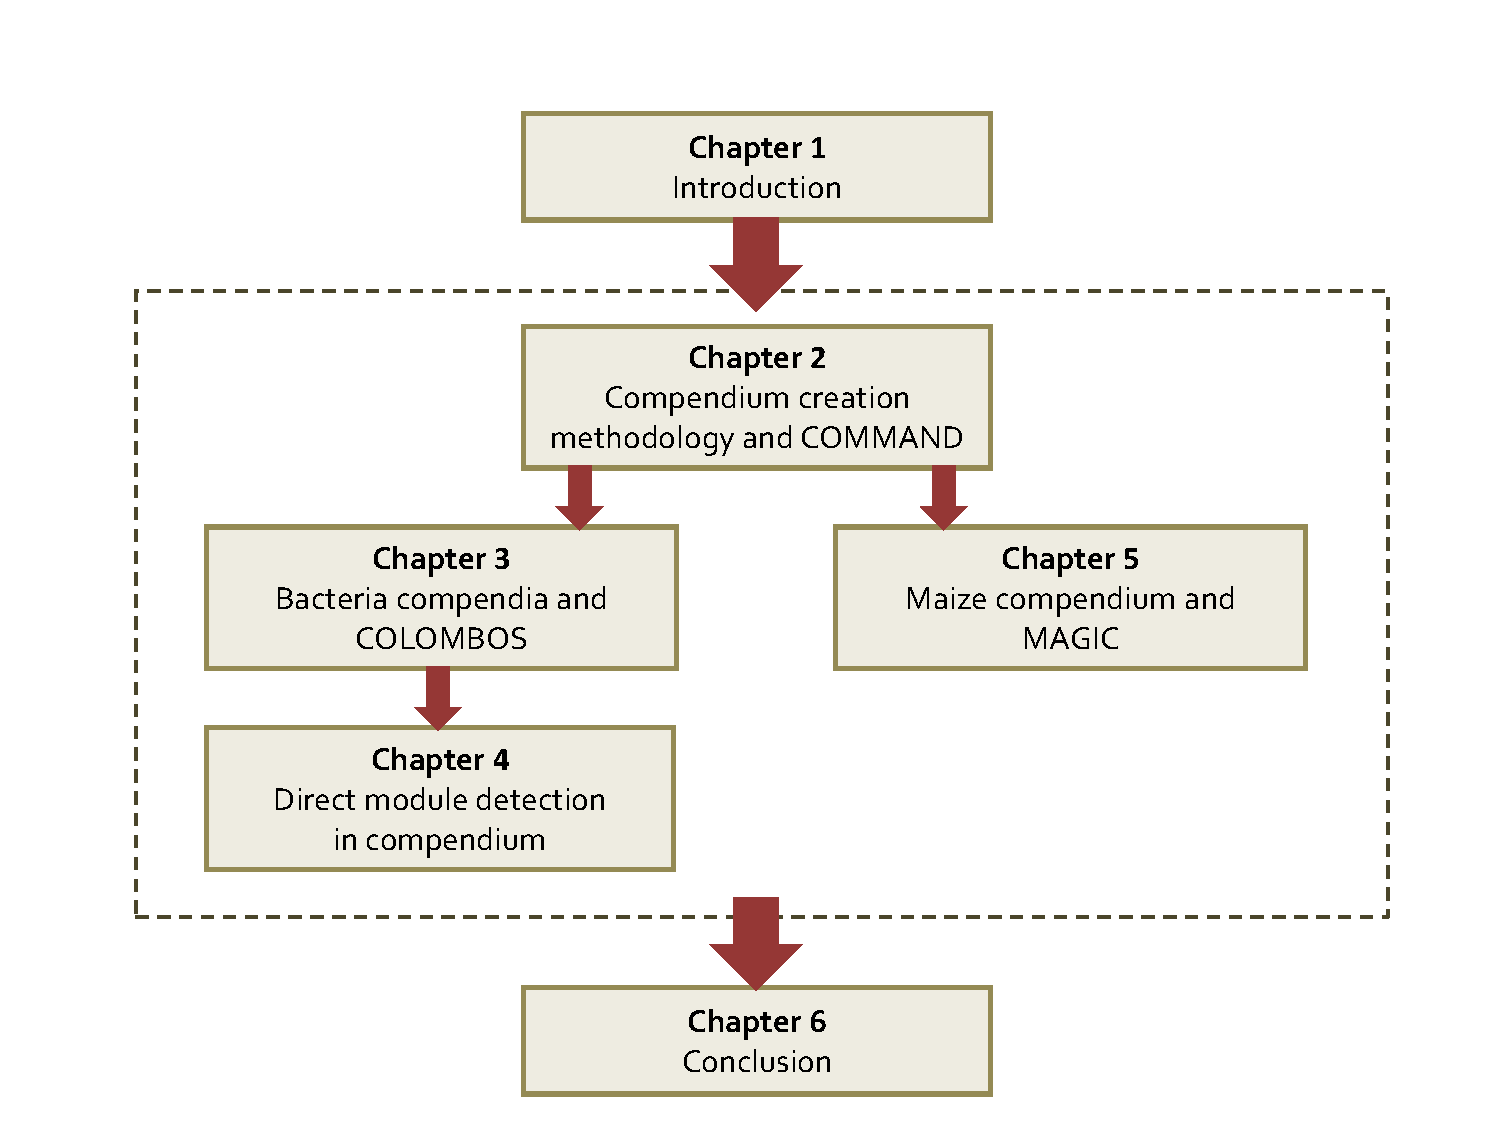
\includegraphics[trim=0cm 0cm 0cm 1cm, clip=true, width=1\textwidth]
                  {thesis_structure.pdf}
  \caption[Organization of the dissertation]{
     \textbf{Organization of the dissertation}}. 
  \label{fig:intro_overview}
\end{figure}
%
Chapter \ref{ch:command} describes the development of a methodology that
enables the creation of an organism-specific cross-platform expression
compendium.
%
We first thoroughly investigated the issues involved in creating
cross-platform compendium, including, the data representation
heterogeneity, particularly for those related to the data generated on
dual-channel microarrays, the lack of standards to specify experimental
meta-data, and the sources of data inconsistency across experiments and
platforms.
%
Based on our study, we conceived a compendium creation methodology
containing three major steps: data collection, annotation, and
homogenization, each of which targets one specific issue identified.
%
To reduce the complexity involved in compendium creation and facilitate
the maintenance of existing ones, we then developed a web system that
provides user friendly interfaces to guide user through various steps of
compendium creation.
%
%% The data collection step focuses on collecting raw expression data
%% overcoming the wide-spread representation heterogeneity in the expression
%% data of different platform origin, which has been the great hurdle
%% preventing the resue of the existing data.
%% %
%% The annotation step aims to provide the consistent and complete
%% specification of experimental factors and sample attributes crucial for
%% data exploration and result interpretation, overcoming the issue of the
%% cryptic and often incomplete descriptions available in the public online
%% repositories.
%% %
%% Additionally, using controlled vocabulary, this annotation is
%% programmatically operable, enabling large scale systematic data analysis.
%% %
%% In the last step, raw data are preprocessed using our in-house pipeline and
%% log-ratios are calculated.  The former procedure improves the data
%% consistency between different experiments, and the latter randers them
%% comparable across different platforms.
%
%% The methodology has the advantage of incorporating far more data into a
%% comsistent data set than existing single-platform one, as demonstrated by
%% the \textit{Escherichia coli} compendium presented in Chapter
%% \ref{ch:colombos}.
%% %
%% And it also makes it feasible to create a sizable compendium for species,
%% in which there are large amount of data of very heterogeneous platform
%% origins and no one dominant platform exists, for example, \textit{Bacil lus
%%   subtilis}, \textit{Salmonel la enterica serovar Typhimurium}, \textit{Zea
%%   mays}.
%% %
%
The methodology lays the foundation of this research work.
%
%
%
In Chapter \ref{ch:colombos}, three such cross-platform compendia for
bacterial model organisms (\textit{Escherichia coli}, \textit{Bacillus
  subtilis}, and \textit{Salmonella enterica} serovar Typhimurium) are
presented together with a web access portal COLOMBOS that incorporates a
suite of intuitive tools for data exploration, analysis and visualization
and provides easy-of-use access to these compendia.
%
The utility of both the compendia and the web portal is demonstrated in a
case study, in which COLOMBOS analysis tools are employed to identify novel
targets for \textit{E. coli} transcription factor FUR (Ferric Uptake
Regulation) based on their expression similarity to that of the known FUR
targets across a range of diverse conditions in \textit{E. coli} compendium.
%
Chapter \ref{ch:distiller} further showcased the utility of the compendium
in the application of query driven condition dependent co-expression module
discovery.
%
Two web services, DISTILLER \cite{Lemmens2009} and COLOMBOS
\cite{Engelen2011}, are recruited to explore \textit{E. coli}
compendium and identify such modules for query gene \textit{sodA}.
%
We demonstrates that the complementarity between the results obtained by
each approach well reflects the complementarity nature of these two
approaches, and the choice of the method depends on the nature of the
biological questions to be answered.
%
%
%
Chapter \ref{ch:magic} describes our attempt to create a
cross-platform expression compendium for eukaryotic organisms utilizing the
methodology.
%
Here, we specifically address two issues: platform probe heterogeneity due
to the lack of the complete genome sequence, and precise biological sample
annotation that manifests the abundant genetic repository (breeding lines)
of maize species and its complex life style (development stage) and
structure (tissue).
%
%
%
At the end, the main achievements of this PhD study are summarized in
Chapter \ref{ch:conclusion} followed by some perspectives for future
research.










% glossary

\glossary{name=GEO, description=Gene Expression Omnibus}
\glossary{name=EBI, description=European Bioinformatics Institute}
\glossary{name=NCBI, description=National Center for Biotechnology Information}


\glossary{name=COLOMBOS, description=Collection of Microarrays for Bacterial 
Organisms}
\glossary{name=DISTILLER, description=Data Integration System to Identify Links 
in Expression Regulation}
\glossary{name=ViTraM, description=VIsualization of TRAnscriptional Modules}
\glossary{name=EcoCyc, description=Encyclopedia of \textit{Escherichia coli} 
K-12 Genes and Metabolism}
\glossary{name=BioCyc, description=Pathway/Genome Databases and Pathway Tools 
Software}
\glossary{name=MaizeGDB, description=Maize Genetics and Genomics Database} 
\glossary{name=PLEXdb, description=Plant Expression Database}
\glossary{name=CORNET, description=CORrelation NETworks}
\glossary{name=BLAST, description=Basic Local Alignment Search Tool}


\glossary{name=PSSM, description=Position Specific Scoring Matrices}
\glossary{name=ChIP, description=Chromatin Immunoprecipitation}
\glossary{name=NGS, description=next generation sequencing}


\glossary{name=DNA, description=deoxyribonucleic acid}
\glossary{name=cDNA, description=complementary deoxyribonucleic acid}
\glossary{name=RNA, description=ribonucleic acid}
\glossary{name=UTR, description=untranslated region}


\glossary{name=iPOP, description=integrative personal omics profile}
\glossary{name=FGS, description=Filtered Gene Set}


\glossary{name=SOFT, description=Simple Omnibus Format in Text}
\glossary{name=GPR, description=GenePix Results format}
%\glossary{name=CEL, description=}
\glossary{name=CDF, description=Chip Description File}
\glossary{name=GPR, description=GenePix Results}
\glossary{name=IDF, description=Investigation Description Format file}
\glossary{name=SDRF, description=Sample and Data Relationship Format file}
\glossary{name=ADF, description=Array Design Format file}
\glossary{name=MAGE-TAB, description=MicroArray Gene Expression Tabular}
\glossary{name=MGED, description=Microarray Gene Expression Databases}
\glossary{name=MIAME, description=Minimum Information About A Microarray 
Experiment}




% nomenclature

\nomenclature{Compendium}{Essentially an expression (log-ratio) value matrix, 
whose rows correspond to the known genes and columns correspond to sample 
contrasts}

\nomenclature{Sub-compendium}{A subset of compendium containing contrasts 
sharing certain properties of interests, e.g., contrasts in which the gene 
expression profiles of different tissues are compared}

\nomenclature{Sample contrast}{Where the expression values of genes from two 
biological samples, one set at the test and the other reference, are compared 
and the expression variations between samples are represented as log ratio}

\nomenclature{Coexpression}{Genes' coherent expression responses to 
certain alterations in the organism's intra- or extracellular environment}

\nomenclature{Coexpression Module}{A combined set of genes and condition 
contrasts, where the coexpression pattern appears}

\nomenclature{Homogenization}{Our methodology to convert raw 
intensity expression values from individual biological sample into expression 
log-ratios between two different biological samples paired as a contrast so 
that they are comparable across different microarray platforms and experiments}

\nomenclature{Coregulation}{A phenomenon that genes are regulated by common 
transcription factor(s)}

\nomenclature{Frequent itemset mining}{A data mining technology tries to 
extract information about a set of items that occurs together frequently}

\nomenclature{Closed itemset}{Frequent itemset that cannot be extended with an
additional item without reducing the number of its occurrences}











%%%%%%%%%%%%%%%%%%%%%%%%%%%%%%%%%%%%%%%%%%%%%%%%%%
% Keep the following \cleardoublepage at the end of this file, 
% otherwise \includeonly includes empty pages.
\cleardoublepage

% vim: tw=70 nocindent expandtab foldmethod=marker foldmarker={{{}{,}{}}}
